\section{Результаты расчетов}

\subsection{IBM Blue Gene/P}

Были проведены расчеты для следующего числа процессоров: 1, 128, 256, 512 на сетках с числом узлов $1000 \times 1000$ и $2000 \times 2000$ без использования \texttt{OpenMP} и с использованием (гибридная программа). Результаты расчетов представлены в таблицах \ref{table:bluegene} и \ref{table:bluegene_omp} соответственно. На рисунках \ref{fig:bluegene_s_1000} и \ref{fig:bluegene_s_2000} представлены графики зависимости ускорения от числа процессоров для решений MPI и MPI+OpenMP для сеток $1000 \times 1000$ и $2000 \times 2000$ точек соответственно.

\begin{table}[H]
  \centering
  \resizebox{\textwidth}{!}{\begin{tabular}{ r | r | r | r }
    \hline
    Число процессоров $N_p$ & Число точек сетки $N^2$ & Время решения $T$, сек & Ускорение S \\
    \hline
    1 & 1000 $\times$ 1000 & 1652.024522 & \\
    128 & 1000 $\times$ 1000 & 12.466822 & 132.514 \\
    256 & 1000 $\times$ 1000 & 4.089699 & 403.948 \\
    512 & 1000 $\times$ 1000 & 3.112727 & 530.732 \\
    \hline
    1 & 2000 $\times$ 2000 & 13587.828157 & \\
    128 & 2000 $\times$ 2000 & 107.145814 & 126.816 \\
    256 & 2000 $\times$ 2000 & 54.971916 & 247.178 \\
    512 & 2000 $\times$ 2000 & 23.605630 & 575.618 \\
    \hline
  \end{tabular}}
  
  \caption{Таблица с результатами расчетов на ПВС <<IBM Blue Gene/P>> без использования \texttt{OpenMP}.}
  \label{table:bluegene}
\end{table}

\begin{table}[H]
  \centering
  \resizebox{\textwidth}{!}{\begin{tabular}{ r | r | r | r }
    \hline
    Число процессоров $N_p$ & Число точек сетки $N^2$ & Время решения $T$, сек & Ускорение S \\
    \hline
    1 & 1000 $\times$ 1000 & 440.038644 & \\
    128 & 1000 $\times$ 1000 & 3.567329 & 123.352 \\
    256 & 1000 $\times$ 1000 & 1.373013 & 320.491 \\
    512 & 1000 $\times$ 1000 & 1.308485 & 336.296 \\
    \hline
    1 & 2000 $\times$ 2000 & 2932.124473 & \\
    128 & 2000 $\times$ 2000 & 24.786318 & 118.296 \\
    256 & 2000 $\times$ 2000 & 13.203982 & 222.064 \\
    512 & 2000 $\times$ 2000 & 7.093203 & 413.371 \\
    \hline
  \end{tabular}}
  
  \caption{Таблица с результатами расчетов на ПВС <<IBM Blue Gene/P>> с использованием \texttt{OpenMP}.}
  \label{table:bluegene_omp}
\end{table}

\begin{figure}[H]
    \centering
    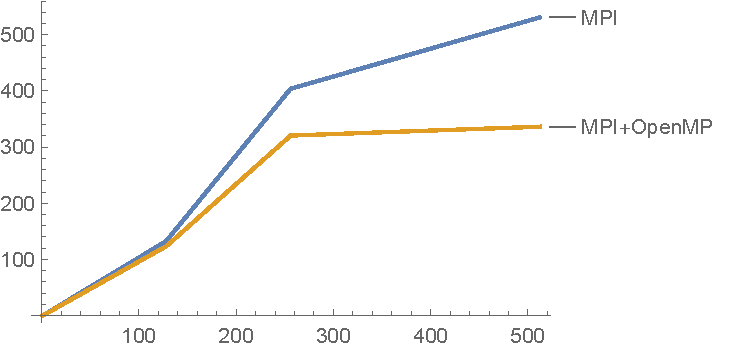
\includegraphics[width=0.8\linewidth]{bluegene_s_1000.pdf}
    \caption{График зависимости ускорения от числа процессоров для решений MPI и MPI+OpenMP для сетки $1000 \times 1000$ точек.}
    \label{fig:bluegene_s_1000}
\end{figure}

\begin{figure}[H]
    \centering
    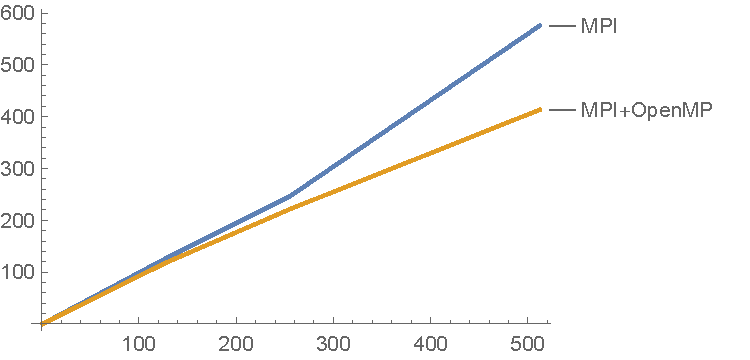
\includegraphics[width=0.8\linewidth]{bluegene_s_2000.pdf}
    \caption{График зависимости ускорения от числа процессоров для решений MPI и MPI+OpenMP для сетки $2000 \times 2000$ точек.}
    \label{fig:bluegene_s_2000}
\end{figure}

\subsection{<<Ломоносов>>}

Были проведены расчеты для следующего числа процессоров: 1, 8, 16, 32, 64, 128 на сетках с числом узлов $1000 \times 1000$ и $2000 \times 2000$. Результаты представлены в таблице \ref{table:lomonosov}.

\begin{table}[H]
  \centering
  \resizebox{\textwidth}{!}{\begin{tabular}{ r | r | r | r }
    \hline
    Число процессоров $N_p$ & Число точек сетки $N^2$ & Время решения $T$, сек & Ускорение S \\
    \hline
    1 & 1000 $\times$ 1000 & 234.741683 & \\
    8 & 1000 $\times$ 1000 & 29.986969 & 7.828 \\
    16 & 1000 $\times$ 1000 & 15.227095 & 15.416 \\
    32 & 1000 $\times$ 1000 & 7.721868 & 30.400 \\
    64 & 1000 $\times$ 1000 & 4.138745 & 56.718 \\
    128 & 1000 $\times$ 1000 & 2.141562 & 109.612 \\
    \hline
    1 & 2000 $\times$ 2000 & 2123.040323 & \\
    8 & 2000 $\times$ 2000 & 238.554619 & 8.900 \\
    16 & 2000 $\times$ 2000 & 120.629342 & 17.600 \\
    32 & 2000 $\times$ 2000 & 60.860912 & 34.884 \\
    64 & 2000 $\times$ 2000 & 30.859959 & 68.796 \\
    128 & 2000 $\times$ 2000 & 15.950209 & 133.104 \\
    \hline
  \end{tabular}}
  
  \caption{Таблица с результатами расчетов на ПВС <<Ломоносов>>.}
  \label{table:lomonosov}
\end{table}

\clearpage
